\documentclass[10pt]{article}
\usepackage{fullpage,enumitem,amsmath,amssymb,graphicx,listings,tikz,bbm,xcolor}
\setlength{\parindent}{0pt}

\begin{document}

{\Large \textbf{Markov Decision Processes}}

\section*{\normalsize Policies}

Recall that the reward for entering an empty cell is -1, a mountainous cell -3, the pond -50, and the goal +100. These are the rewards defined according to the environment. However, if our robot wanted to move from one cell to another, it it not guaranteed to succeed. Therefore, we must calculate the expected reward, which takes into account not just the rewards set by the environment, but the robot's transition model too.
	
	\begin{figure}[h!]
		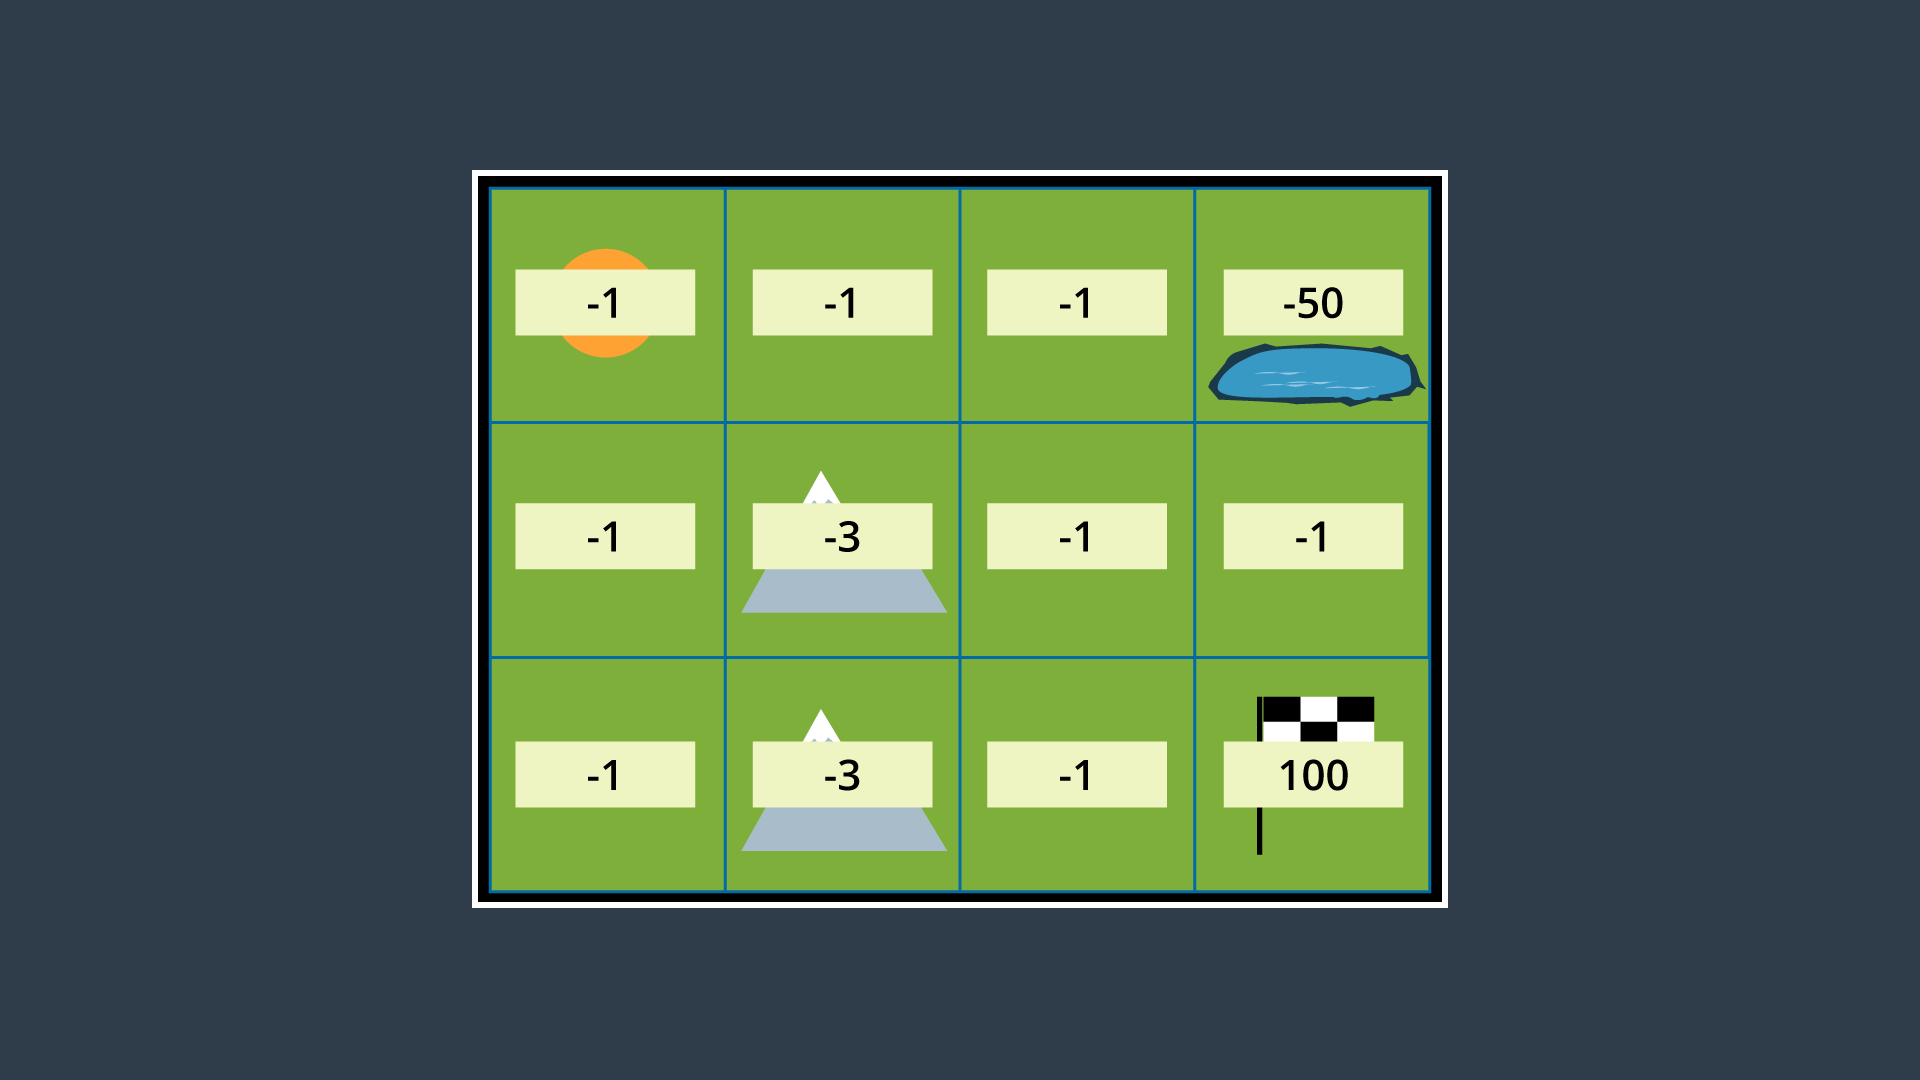
\includegraphics[width=\linewidth]{Images/mdp1.png}
		\caption{Rewards}
	\end{figure}
	
	\begin{figure}[h!]
		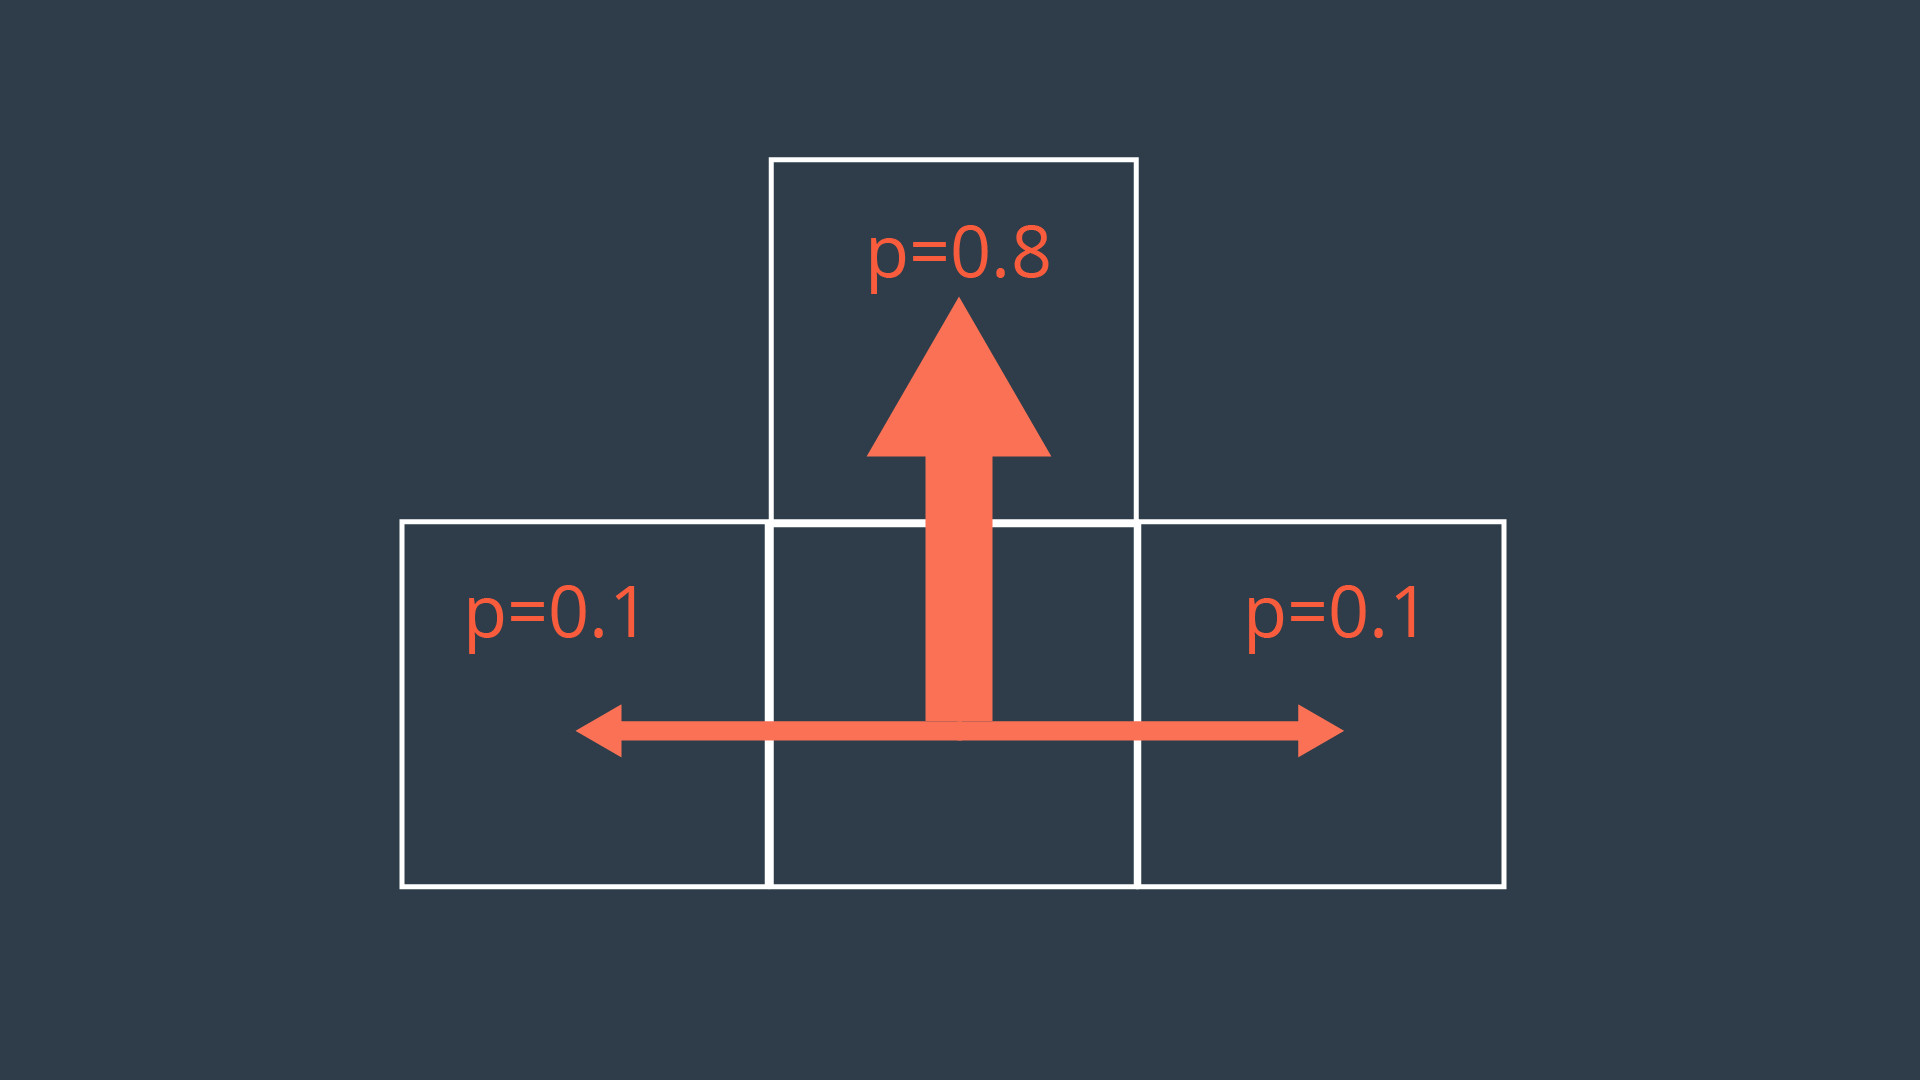
\includegraphics[width=\linewidth]{Images/mdp0.png}
		\caption{Robot Transition Model}
	\end{figure}
	
	\begin{figure}[h!]
		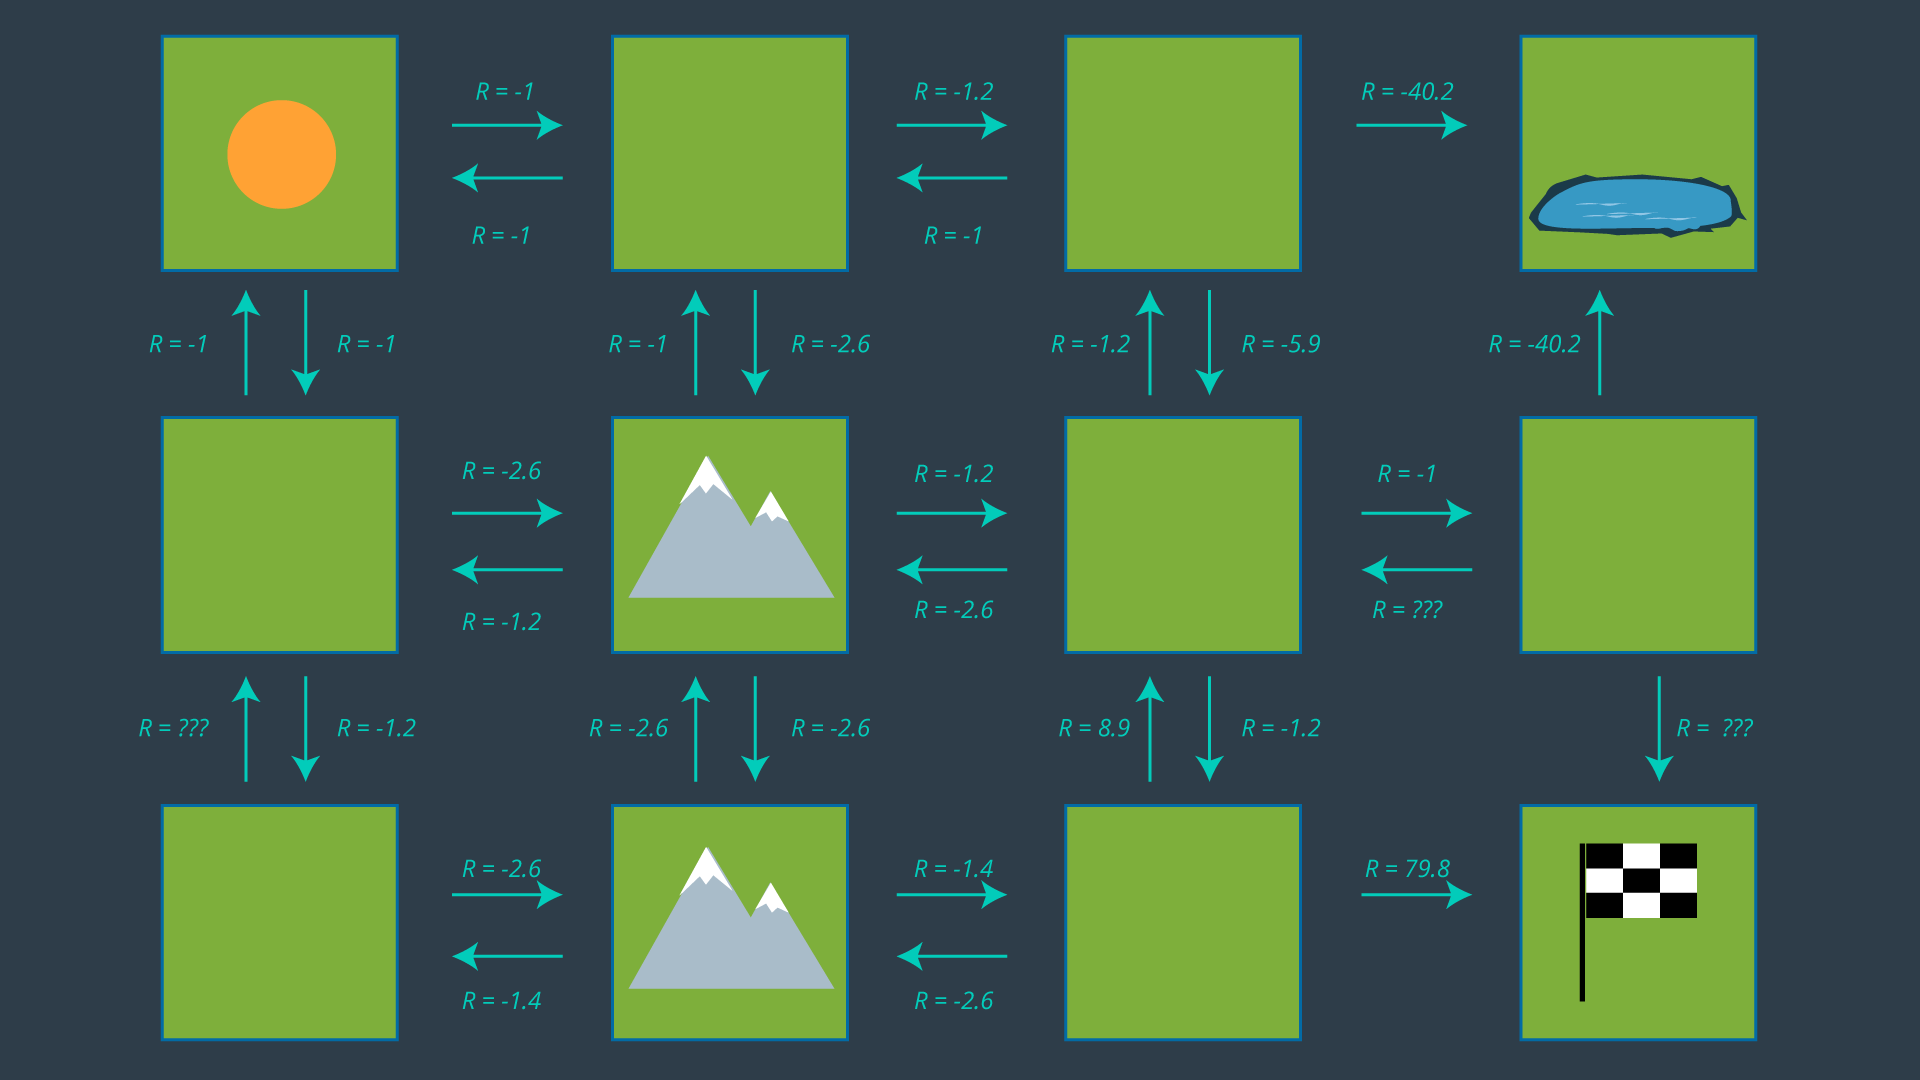
\includegraphics[width=\linewidth]{Images/mdp2.png}
		\caption{Expected Rewards}
	\end{figure}
	
\begin{enumerate}
	\item What is the expected reward for moving from the bottom-left cell to the cell above it?
	
	\begin{align*}
	expected\,reward &= 0.8 * (-1) + 0.1 * (-1) + 0.1 * (-3)\\
	&= -1.2
	\end{align*}
	
	\item What is the expected reward for moving from the empty cell on the right to the goal,one cell below it?
	
	\begin{align*}
	expected\,reward &= 0.8 * (100) + 0.1 * (-1) + 0.1 * (-1)\\
	&= 79.8
	\end{align*}
	
	\item What is the expected reward for moving from the empty cell on the right to the cell to its left?
	
	\begin{align*}
	expected\,reward &= 0.8 * (-1) + 0.1 * (-50) + 0.1 * (100)\\
	&= 4.2
	\end{align*}
	
\end{enumerate}

\section*{\normalsize State Utility}

	\begin{figure}[h!]
		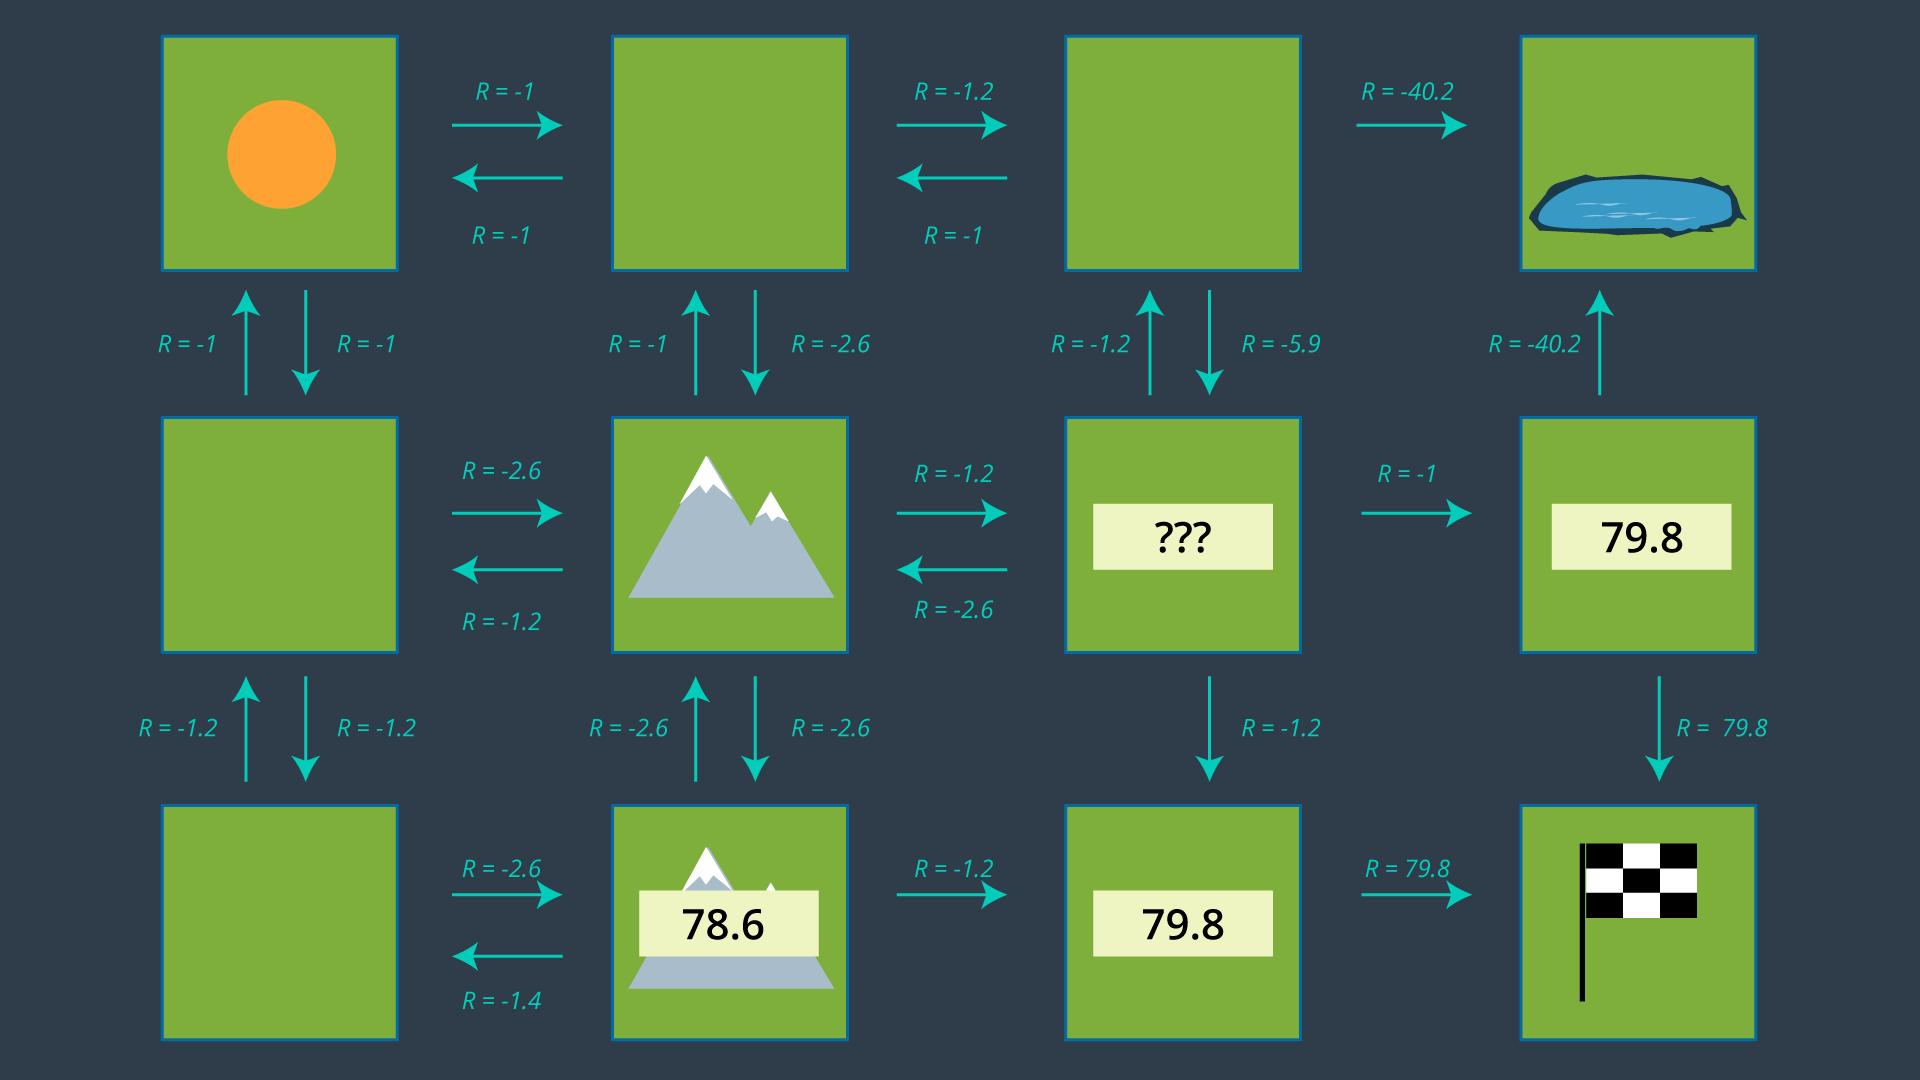
\includegraphics[width=\linewidth]{Images/mdp3.png}
		\caption{Utility}
	\end{figure}
	
\begin{enumerate}
	\item What is the utility of the state to the right of the center mountain following the optimal policy?
	$$U^\pi(s) = 78.8$$
	
\end{enumerate}

\end{document}